\documentclass[tikz,border=8pt]{standalone}
% Requer xelatex e a fonte Poppins. Ajuste o Path abaixo (ou use \setmainfont{Poppins} se ela estiver instalada).
\usepackage{fontspec}
\setmainfont{Poppins}[Path=/usr/share/fonts/truetype/google-fonts/,Extension=.ttf,UprightFont=*-Regular,BoldFont=*-Bold,ItalicFont=*-Italic,BoldItalicFont=*-BoldItalic]
\usepackage{xcolor}
\definecolor{azulescuro}{HTML}{4A6F9C}
\definecolor{azulmedio}{HTML}{6F93BC}
\definecolor{azulclaro}{HTML}{E9EDF3}
\definecolor{azulsenac}{HTML}{1F4E9A}
\definecolor{laranja}{HTML}{F19E37}
\definecolor{laranjaescuro}{HTML}{D9731A}
\definecolor{laranjaclaro}{HTML}{FDEFD9}
\definecolor{cinzatitulo}{HTML}{333333}
\definecolor{cinzatexto}{HTML}{5C5C5C}
\usepackage{tikz}
\usetikzlibrary{positioning,arrows.meta,fit,backgrounds,calc}

\definecolor{favorfraco}{HTML}{CBD8E8}
\definecolor{favormedio}{HTML}{9FB6D3}
\definecolor{favorforte}{HTML}{4A6F9C}
\definecolor{contra}{HTML}{F5C98A}
\begin{document}
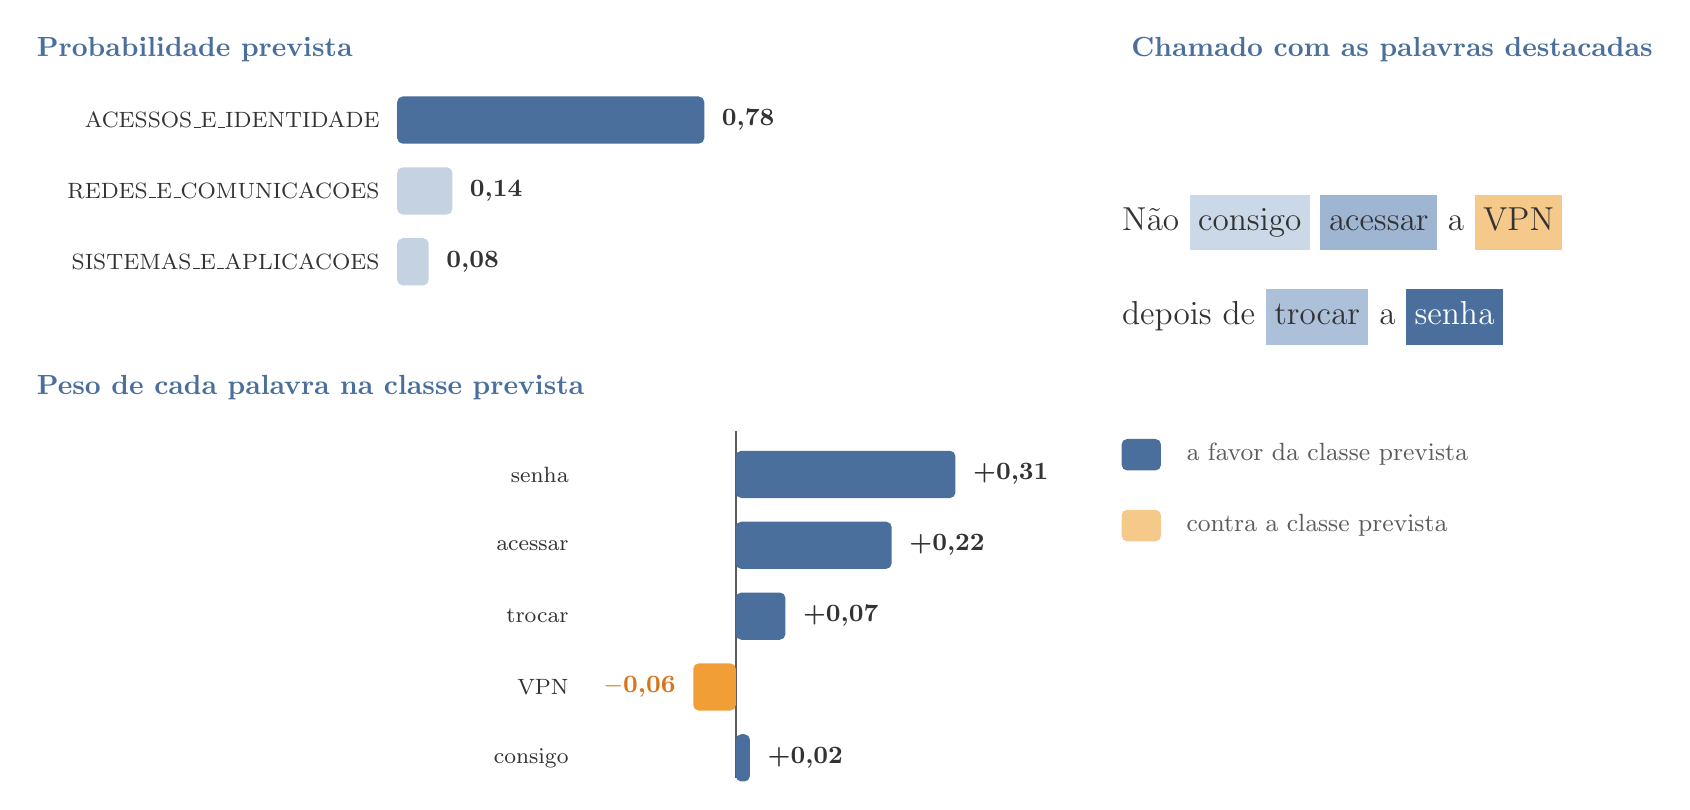
\begin{tikzpicture}[font=\small\color{cinzatexto}]
% ---------- probabilidade prevista
\node[font=\normalsize\bfseries\color{azulescuro}, anchor=west] at (-4.6,0.9) {Probabilidade prevista};
\def\W{5.0}
\foreach \y/\nome/\p/\cor/\rot in {0/{ACESSOS\_E\_IDENTIDADE}/0.78/azulescuro/{0,78}, -0.9/{REDES\_E\_COMUNICACOES}/0.14/azulclaro!70!azulmedio/{0,14}, -1.8/{SISTEMAS\_E\_APLICACOES}/0.08/azulclaro!70!azulmedio/{0,08}}{
  \node[anchor=east, font=\footnotesize\color{cinzatitulo}] at (0,\y) {\nome};
  \fill[\cor, rounded corners=2pt] (0.1,\y-0.3) rectangle (0.1+\p*\W,\y+0.3);
  \node[anchor=west, font=\small\bfseries\color{cinzatitulo}] at (0.2+\p*\W,\y) {\rot};
}
% ---------- pesos
\node[font=\normalsize\bfseries\color{azulescuro}, anchor=west] at (-4.6,-3.4) {Peso de cada palavra na classe prevista};
\def\z{4.4} % posição do zero
\def\k{9}   % escala cm por unidade
\draw[cinzatexto, line width=0.6pt] (\z,-3.95) -- (\z,-8.35);
\foreach \y/\nome/\v/\txt in {-4.5/senha/0.31/{+0,31}, -5.4/acessar/0.22/{+0,22}, -6.3/trocar/0.07/{+0,07}, -7.2/VPN/-0.06/{$-$0,06}, -8.1/consigo/0.02/{+0,02}}{
  \node[anchor=east, font=\footnotesize\color{cinzatitulo}] at (\z-2.0,\y) {\nome};
  \pgfmathsetmacro{\x}{\z+\v*\k}
  \pgfmathparse{\v>0 ? 1 : 0}\ifnum\pgfmathresult=1
    \fill[azulescuro, rounded corners=2pt] (\z,\y-0.3) rectangle (\x,\y+0.3);
    \node[anchor=west, font=\small\bfseries\color{cinzatitulo}] at (\x+0.1,\y) {\txt};
  \else
    \fill[laranja, rounded corners=2pt] (\x,\y-0.3) rectangle (\z,\y+0.3);
    \node[anchor=east, font=\small\bfseries\color{laranjaescuro}] at (\x-0.1,\y) {\txt};
  \fi
}
% ---------- chamado destacado
\def\xc{9.3}
\node[font=\normalsize\bfseries\color{azulescuro}, anchor=west] at (\xc,0.9) {Chamado com as palavras destacadas};
\node[anchor=west, text=cinzatitulo, font=\large, inner sep=0pt] (l1) at (\xc,-1.3)
  {Não \colorbox{favorfraco}{\strut consigo} \colorbox{favormedio}{\strut acessar} a \colorbox{contra}{\strut VPN}};
\node[anchor=west, text=cinzatitulo, font=\large, inner sep=0pt] (l2) at (\xc,-2.5)
  {depois de \colorbox{favormedio!70!favorfraco}{\strut trocar} a \colorbox{favorforte}{\strut\color{white} senha}};
% legenda
\fill[favorforte, rounded corners=2pt] (\xc,-4.45) rectangle ++(0.5,0.4);
\node[anchor=west, font=\small\color{cinzatexto}] at (\xc+0.7,-4.25) {a favor da classe prevista};
\fill[contra, rounded corners=2pt] (\xc,-5.35) rectangle ++(0.5,0.4);
\node[anchor=west, font=\small\color{cinzatexto}] at (\xc+0.7,-5.15) {contra a classe prevista};
\end{tikzpicture}
\end{document}
